\documentclass[notes=hide,hyperref={dvipdfmx,pdfpagelabels=false}]{beamer}
\mode<article>
{
  \usepackage{fullpage}
  \usepackage{pgf}
  \usepackage[xetex]{hyperref}
  \setjobnamebeamerversion{beamer}
}

\mode<presentation>
{
  %\usetheme{Frankfurt}
 %\usetheme{My}
  \usetheme{Madrid}
  % or ...
%\usecolortheme{seagull}
  %\setbeamercovered{transparent}
  %\setbeamercovered{dynamic}
  % or whatever (possibly just delete it)
}
\usenavigationsymbolstemplate{}
\usefonttheme{structurebold}
\usepackage{multimedia}
%\usepackage{tikz}
\usepackage{fontspec,xunicode,xltxtra}

%\usepackage{polyglossia}
%\setdefaultlanguage[spelling=new, latesthyphen=true]{german}
%\setsansfont{DejaVu Sans}
%\setsansfont{Verdana}
%\setsansfont{Arial}
%\setromanfont{Linux Libertine O}
%\setsansfont{Linux Biolinum O}

\setbeamertemplate{footline}
{
\leavevmode
%\hbox{\begin{beamercolorbox}[wd=.5\paperwidth,ht=2.5ex,dp=1.125ex,
%leftskip=.3cm plus1fill,rightskip=.3cm]{author in head/foot}%
%    \usebeamerfont{author in head/foot}\insertshortauthor
%  \end{beamercolorbox}%
%  \begin{beamercolorbox}[wd=.5\paperwidth,ht=2.5ex,dp=1.125ex,leftskip=.3cm,
%rightskip=.3cm plus1fil]{title in head/foot}%
%    \usebeamerfont{title in head/foot}\insertshorttitle\hfill

\hfill\insertframenumber  \hspace{3pt}

%\inserttotalframenumber
%\hspace*{2ex}
%  \end{beamercolorbox}}%
  \vskip3pt%
}

\usepackage[ngerman]{babel}
\selectlanguage{ngerman}

%
% math/symbols
%
\usepackage{amssymb}
\usepackage{amsthm}
% \usepackage{latexsym}
\usepackage{amsmath}
%\usepackage{amsxtra} %Weitere Extrasymbole
%\usepackage{empheq} %Gleichungen hervorheben
%\usepackage{bm}
 %\bm{A} Boldface im Mathemodus

\usepackage{cellspace}
\setlength{\cellspacetoplimit}{2pt}
\setlength{\cellspacebottomlimit}{2pt}

%%%%%%%%%%%%%%%%%% Fuer Frames [fragile]-Option verwenden!
%Programm-Listing
%%%%%%%%%%%%%%%%%%
%Listingsumgebung fuer verbatim
%Grauhinterlegeter Text
%Automatischer Zeilenumbruch ist aktiviert
\usepackage{listings}
\definecolor{lgray}{gray}{0.80}
%\lstset{backgroundcolor=\color{lgray}, frame=single, basicstyle=\ttfamily, breaklines=true}
\lstnewenvironment{sage}{\lstset{backgroundcolor=\color{lgray},language=Python, emphstyle=\color{red}, frame=single, basicstyle=\ttfamily, breaklines=true,mathescape =true,escapechar=§}}{}


\usepackage{mydef}
%\usepackage{cmap} % you can search in the pdf for umlauts and ligatures
\usepackage{colonequals} %corrects the definition-symbols \colonequals (besides others)
\title{Einführung in Sage}
%
%\subtitle{Disputation} % (optional)

\author{Jochen Schulz}
% - Use the \inst{?} command only if the authors have different
%   affiliation.

\institute{Georg-August Universit\"at G\"ottingen \pgfimage[height=0.5cm]{../figures/unilogo3}}
% - Use the \inst command only if there are several affiliations.
% - Keep it simple, no one is interested in your street address.

\date{\today}

\subject{Sage}
% This is only inserted into the PDF information catalog. Can be left
% out. 

% If you have a file called "university-logo-filename.xxx", where xxx
% is a graphic format that can be processed by latex or pdflatex,
% resp., then you can add a logo as follows:

%\logo{\pgfimage[height=0.5cm]{figures/unilogo3}}


% Delete this, if you do not want the table of contents to pop up at
% the beginning of each subsection:

\AtBeginSection[]
{
  \begin{frame}<beamer>
    \frametitle{Aufbau}
    \tableofcontents[currentsection,currentsubsection]
  \end{frame}
}

\AtBeginSubsection[]
{
  \begin{frame}<beamer>
    \frametitle{Aufbau}
    \tableofcontents[currentsection,currentsubsection]
  \end{frame}
}



%%%%%%%%%%%%%%%%%%%
%Neue Definitionen
%%%%%%%%%%%%%%%%%%%

%Newcommands
\newcommand{\Fun}[1]{\mathcal{#1}}      %Mathcal fuer Funktoren
\newcommand{\field}[1]{\mathbb{#1}}     %Grundkoerper ?? in mathds

\newcommand{\A}{\field{A}}              %Affines A
\newcommand{\C}{\field{C}}              %Complexes C
\newcommand{\Fp}{\field{F}_{\!p}}       %Endlicher Koerper mit p Elementen
\newcommand{\Fq}{\field{F}_{\!q}}       %Endlicher Koerper mit q Elementen
\newcommand{\Ga}{\field{G}_{a}}         %Add Gruppenschema
\newcommand{\K}{\field{K}}              %Generischer Koerper 
\newcommand{\N}{\field{N}}              %Nat Zahlen
\newcommand{\Pj}{\field{P}}             %Projektives P
\newcommand{\R}{\field{R}} 		%Reelle Zahlen
\newcommand{\Q}{\field{Q}}              %Rationale Zahlen  
\newcommand{\Qt}{\field{H}}             %Quaternionen 
\newcommand{\V}{\field{V}}              %Vektorbuendel V
\newcommand{\Z}{\field{Z}}              %Ganze Zahlen

\newcommand{\fdg}{\;|\;}                 %fuer die gilt

%Operatoren
\DeclareMathOperator{\Abb}{Abb}
%\usepackage{sagetex}

\begin{document}
\lstset{basicstyle={\lstbasicfont\footnotesize}}


\subtitle{Einheit 1}
\maketitle

%%%%%%%%%%%%%%%%%%%%%%%%%%%%%%%%%%%%%%
\section*{Organisatorisches}
%%%%%%%%%%%%%%%%%%%%%%%%%%%%%%%%%%%%%

\begin{frame}{Organisatorisches}
\begin{itemize}
\item Anmeldungen zu der Veranstaltung über StudIP \\
      \url{https://www.studip.uni-goettingen.de/}

{\color{blue}{Einführung in Sage (Mathematische Anwendersysteme) (WS 2009/2010)}}
\item Alle Unterlagen (Aufgabenblätter, Vorlesungsfolien, Beispiele, Musterlösungen) können von der  StudIP-Seite (Reiter Dateien) heruntergeladen werden 
\pause
\begin{block}{Dozent}
Jochen Schulz\\
NAM, Zimmer 04 (Erdgescho{\ss})\\
Telefon: 39-4525
Email: \url{schulz@math.uni-goettingen.de}\\
XMPP: \url{schulz@jabber.num.math.uni-goettingen.de}\\

\end{block}
\end{itemize}
\end{frame}

\begin{frame}{Starten des Programms}
\textbf{Vor.:} Account im CIP-Pool der Mathematischen Fakultät (MI und NAM): Registrierungs-Formular unter \url{https://ldap.math.uni-goettingen.de} (\alert{Stud.It-Account} nötig!)\\
\textbf{Wiki} (\url{https://wiki.math.uni-goettingen.de/mediawiki})
\begin{itemize}
\item Sage ist in Version 4.2.1 auf allen Rechnern der Mathematischen Fakultät installiert
\item login direkt oder per \alert{nxclient}
auf den Rechnern \texttt{s1.math.uni-goettingen.de} bis \texttt{s8.math.uni-goettingen.de}
und \texttt{s241.math.uni-goettingen.de} bis \texttt{s245.math.uni-goettingen.de}
\item Starten von Sage: Im Terminal 
\begin{itemize}
 \item \texttt{sage} (Notebook)
\item \texttt{sagetext}  (Textversion)
\end{itemize}
\end{itemize}
\end{frame}

\begin{frame}{Ablauf der Veranstaltung}
\begin{itemize}
\item Blockveranstaltung vom  15.2.-26.2.2010
\item Vorlesung: 9.15 Uhr bis 11.30 Uhr
\item Nachmittags: 4 Übungsgruppen \`a je 1h 15min
\begin{itemize}
\item 13:00-14:15 (Tutor: J. Schulz)	
\item 14:15-15:30 (Tutor: C. Rügge)
\item 15:30-16:45 (Tutor: J. Schulz)
\item 16:45-18:00 (Tutor: C. Rügge)
\end{itemize}

\item Scheinerwerb
\begin{itemize}
\item Regelmäßige Teilnahme an den Übungen
\item Projektarbeit durchführen
\item Klausur am 1.3.2009; 10:00 - 12:00; Anmeldung über FlexNow!
\end{itemize}
\end{itemize}
\end{frame}

\begin{frame}[<+->]{Inhalt der Vorlesung}
\begin{description}
 \item[1. Tag]Organisatorisches, Aufbau von Sage, Streifzug durch Sage
\item [2. Tag]Grundlagen Sage (grundlegende Datentypen, Ausdrücke), Lösen von Gleichungen, Symbolisches Rechnen
\item [3. Tag] Mengen,  natürliche, rationale, reelle und komplexe Zahlen, Gleitkommazahlen, Ungleichungen
\item [4. Tag] Vektoren und Matrizen, Lineare Algebra in Sage, Programmieren I
\item [5. Tag] Datencontainer in Sage, Lineare Abbildungen und Matrizen
\item [6. Tag] Folgen und Reihen
\item [7. Tag] Reelle Funktionen, Grafiken
\item [8. Tag] Differenzial- und Integralrechnung
\item [9. Tag] Grundlagen der Programmierung,  Zeichenketten (Strings)
\item [10. Tag] Fragestunde
\end{description}
\end{frame}

\begin{frame}{Aufbau}
\tableofcontents
\end{frame}



%%%%%%%%%%%%%%%%%%%%%%%%%%%%%%
\section{Was ist Sage?}
%%%%%%%%%%%%%%%%%%%%%%%%%%%%%%%%%

\begin{frame}{Computeralgebra-Systeme}

\begin{block}{Computeralgebra}
beschäftigt sich mit \alert{exakten} Berechnungen von
mathematischen Objekten
\end{block}
\bigskip

\begin{block}{Mathematische Objekte} 
Natürliche Zahlen, reelle Zahlen, Polynome, Funktionen,
Gruppen, Ringe, \ldots
\end{block}

\begin{block}{Numerischen Berechnungen}
Bei numerischen
Rechnungen (z.B. Taschenrechner) benutzt man Zahlen in 
{\color{blue}Gleitpunktdarstellung}, also i.A.~nur Näherungen an die
gesuchte Lösung
\end{block}
\end{frame}

\begin{frame}{Computeralgebra != Numerische Berechnung}
\begin{block}{Beispiel}
\begin{tabular}{ll}
 Mathematische Objekte & $\pi$, $\sqrt{2}$\\
 Gleitpunktdarstellung (8 Stellen)& $3.1415927$, $1.4142136$
\end{tabular}
\end{block}
\end{frame}

\begin{frame}{Computeralgebra-Systeme}
\begin{small}
\begin{block}{Allgemein}
\begin{tabular}{ll}
\alert{Sage} & Schnittstelle für Mathematik-Software \\
 \alert{LiveMath} &Maple\\
 \alert{Maxima} &Free, GPL, von Sage benutzt\\
\alert{Mathematica} &Platzhirsch\\
 \alert{Maple} &Platzhirsch\\
\alert{Matlab/Octave} &Für große Rechnungen, inkl. Mupad\\
\alert{Magma} &Spezielle mathematische Rechungen\\
 \alert{SymPy} &Phython-Bibliotheken als CAS-Verwendbar\\
 \alert{SymbolicC++} &Bibliotheken zur CA in C++
\end{tabular}

Überblick:{\scriptsize
\url{http://en.wikipedia.org/wiki/Comparison_of_computer_algebra_systems} }
\end{block}

%\alert{Spezialanwendungen}: & Cadabra (Körpertheorie)\\
%& PARI/GP (Zahlentheorie, Teil von Sage)\\
%& GAP (Gruppentheorie, Teil von Sage) \\
%& Macaulay (Algebraische Geometrie)\\
%& Singular (Algebraische Geometrie, Teil von Sage)
%\end{tabular}
\end{small}
\end{frame}

\begin{frame}{Sage}
\begin{itemize}
\item Open-source (GPL) Mathematik Software System.
%\begin{itemize}
% \item Entwicklung von MuPAD seit 1990 an der Universität Paderborn
% \item Seit 1997 Teilausgliederung in die SciFace Sofware GmbH
% \item MuPAD wurde mitte des Jahres 2008 an Mathworks verkauft
% \item MuPAD ist seither eine Toolbox des Programms \alert{Matlab} (Symbolic Toolbox)
%\end{itemize}
\item Alternative zu den 4 M's: Magma, Maple, Mathematica, Matlab.
\item Basiert auf Python.
\item Objektorientiert.
\item Besitzt Frontends für viele externe Software $\rightarrow$ Synergie-Effekte
\end{itemize}
\end{frame}


\begin{frame}{}
von Joachim Neubüser (Gründer von GAP):
 \begin{small}
\begin{quote}
    You can read Sylow’s Theorem and its proof [. . . ] and then
    you can use Sylow’s Theorem for the rest of your life free of
    charge, but for many computer algebra systems license fees
    have to be paid regularly [. . . ]. You press buttons and you get
    answers in the same way as you get the bright pictures from
    your television set but you cannot control how they were
    made in either case. 

With this situation two of the most basic rules of conduct in
mathematics are violated: in mathematics information is
passed on free of charge and everything is laid open for
checking. Not applying these rules to computer algebra
systems that are made for mathematical research [. . . ]
means moving in a most undesirable direction. Most
important: can we expect somebody to believe a result of a
program that he is not allowed to see?  
\end{quote}
 \end{small}

\end{frame}




\begin{frame}[<+->]{Sage - Stärken und Schwächen}
\alert{Stärken}
\begin{itemize}
\item interaktiver Quellcode-Debugger
\item umfangreiches Hilfesystem
\item Einfaches Einbinden von C/C++ Routinen (dynamische Module)
\item Schnittstelle zu vielen anderen CAS (Maxima, Pari,
GAP, R, Magma, ..., wovon einige bereits bei Sage enthalten sind)
\item Viele freie (Unterrichts-)materialien im Netz 
\end{itemize}
\alert{Schwächen}
\begin{itemize}
\item Befehlsumfang nicht so mächtig wie bei Maple oder Mathematica
\item es fehlt eine gute Entwicklungsumgebung
\end{itemize}
\end{frame}

%\begin{frame}{Struktur von Sage}
%\begin{center}
%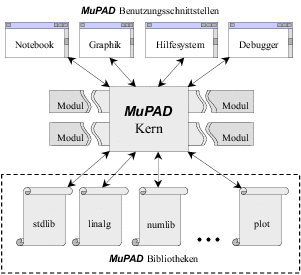
\includegraphics[width=6cm]{figures/components.png}
%\end{center}
%\end{frame}

\begin{frame}{Kern von Sage}
\begin{itemize}
\item \alert{Parser:} Liest die Eingaben und überprüft die Syntax;
  Umwandlung in MuPAD-Datentyp
\item \alert{Auswerter:} Auswertung und Vereinfachung der
  Ergebnisse
\item \alert{Speicherverwaltung:} (MAMMUT $\equiv$ Memory
  Allocation Managment Unit) interne Verwaltung der
  MuPAD-Objekte
\item \alert{Kernfunktionen:}  Oft benötigte Funktionen
  werden aus Effizienzgründen im Kern auf C-Ebene implementiert.
\end{itemize}
\end{frame}

%\begin{frame}{Literatur}
%\begin{itemize}
%\item K. Gehrs, F. Postel. MuPAD -- Eine praktische
%  Einführung. SciFace. 2001.
%\item Ch. Creutzig, J. Gerhard, W. Oevel, St. Wehmeier. Das MuPAD
%  Tutorium. Springer. 2. Auflage. 2002.
%\item M. Majewski. MuPAD Pro Computing Essentials. Springer. 2002.
%\item Rolf Monnerjahn. Mathematische Anwendungen in Biologie, Chemie, Physik. MuPad im Mathematikunterricht: 5.-10. Schuljahr
%\item  Gerd Rapin, Thomas Wassong, Stefan Wiedmann und Stefan Koospal. MuPAD: Eine Einführung
%\end{itemize}
%\end{frame}

%%%%%%%%%%%%%%%%%%%%%%%%%%%%%%%%%%
\section{Streifzug durch Sage}
%%%%%%%%%%%%%%%%%%%%%%%%%%%%%%%%%

\begin{frame}[fragile]{Sage als Taschenrechner}
Hier einige Beispiele:
\begin{sage}
>> 3+4*10+12 
\end{sage}
\begin{sage}
  55 
\end{sage}
\begin{sage}
>> sin(pi) 
\end{sage}
\begin{sage}
  0
\end{sage}
\begin{sage}
>> float(Pi)
\end{sage}
\begin{sage}
  3.14159265358979
\end{sage}
\begin{sage}
>> float(sqrt(2))
\end{sage}
\begin{sage}
  1.41421356237310
\end{sage}
\end{frame}



%%%%%%%%%%%%%%%%%%%%%%%%%%%%%%
\subsection{Eine Kurvendiskussion}
%%%%%%%%%%%%%%%%%%%%%%%%%%%%%%%%%

\begin{frame}[fragile]{Kurvendiskussion I}
Betrachte die durch die reelle Zahl $a$ parametrisierte Funktionenschar:
\[ 
f: x \quad \mapsto \quad \frac{2x^2-20x+42}{x-1}+a, \quad
a \in \mathbb{R} 
\]

\begin{itemize}
\item Eingabe der Funktion
\begin{sage}
>> var('a')
>> f(x) = (2*x^2-20*x +42)/(x-1)+a
\end{sage}
\begin{sage}
  x |--> a + 2*(x^2 - 10*x + 21)/(x - 1)
\end{sage}
\end{itemize}
\end{frame}

\begin{frame}[fragile]{Kurvendiskussion II}
\begin{itemize}
\item Pol ?
\begin{sage}
>> f.limit(x=1, dir='minus')
\end{sage}
\begin{sage}
  x |--> -Infinity
\end{sage}
\begin{sage}
>> f.limit(x=1, dir='plus') 
\end{sage}
\begin{sage}
  x |--> +Infinity
\end{sage}
\item Umformen
\begin{sage}
>> f.full_simplify()
\end{sage}
\begin{sage}
x |--> ((a - 20)*x + 2*x^2 - a + 42)/(x - 1)
\end{sage}
\end{itemize}
\end{frame}

\begin{frame}[fragile]{Kurvendiskussion III}
\begin{itemize}
\item Nullstellen
\begin{sage}
>> solve(f==0,x)
\end{sage}
\begin{scriptsize}
\begin{sage}
[x == -1/4*a - 1/4*sqrt(a^2 - 32*a + 64) + 5, x == -1/4*a + 1/4*sqrt(a^2 - 32*a + 64) + 5]
\end{sage}
\end{scriptsize}
\item Berechnen der Ableitung
\begin{sage}
>> f.differentiate(x)
\end{sage}
\begin{sage} 
x |--> 4*(x - 5)/(x - 1) - 2*(x^2 - 10*x + 21)/(x - 1)^2
\end{sage}
\end{itemize}
\end{frame}

\begin{frame}[fragile]{Kurvendiskussion IV}
\begin{itemize}
\item Extremwerte
\begin{sage}
>> solve(f.differentiate(x)==0,x)
\end{sage}
\begin{sage}
[x == -2*sqrt(3) + 1, x == 2*sqrt(3) + 1]
\end{sage}
\item Lokale Minima und Maxima
\begin{sage}
>> float( ((f.diff(x)).diff(x))(-2*sqrt(3)+1) )
\end{sage}
\begin{sage}
-1.1547005383792501
\end{sage}
\begin{sage}
>> float( ((f.diff(x)).diff(x))(2*sqrt(3)+1) )
\end{sage}
\begin{sage}
1.1547005383792515
\end{sage}
\end{itemize}
\end{frame}

\begin{frame}[fragile]{Kurvendiskussion V}
\begin{itemize}
\item Verhalten von $f$ für große $x$
\begin{sage}
>> f.limit(x=oo); f.limit(x=-oo)
\end{sage}
\begin{sage}
x |--> +Infinity
x |--> -Infinity
\end{sage}
\item Definiere $f_{0}$, $f_{1}$, $f_{2}$
\begin{sage}
>>  f0 = f(x, a=0)
>>  f1 = f(x, a=-20)
>>  f2 = f(x, a=20);f0,f1,f2
\end{sage}
\begin{scriptsize}
\begin{sage}
(2*(x^2 - 10*x + 21)/(x - 1), 2*(x^2 - 10*x + 21)/(x - 1) - 20, 2*(x^2 - 10*x + 21)/(x - 1) + 20)
\end{sage}
\end{scriptsize}
\end{itemize}
\end{frame}

\begin{frame}[fragile]{Plot}
\begin{sage}
p = plot(f0,detect_poles='show',xmin=0, xmax=10,color='red')
p += plot(f1,detect_poles='show',xmin=0, xmax=10,color='green')
p += plot(f2,detect_poles='show',xmin=0, xmax=10,color='blue'); p.show(ymin=-80, ymax=80)
\end{sage}
\begin{center}
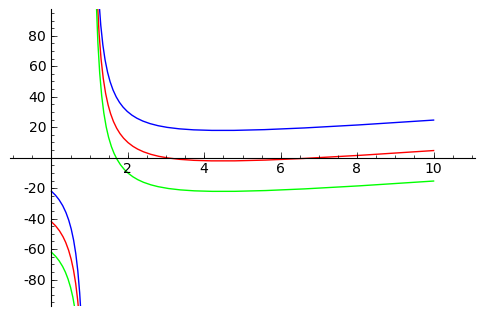
\includegraphics[height=4.5cm]{figures/graphen}
\end{center}
\end{frame}

\begin{frame}[fragile]{Zusammenfassung}
\begin{itemize}
\item Definieren von Variablen mit {\color{blue}'='}, z.B. {\verb~a=3~} 
\item Definieren von Funktionen mit{\color{blue} '='}, z.B. {\verb~f(x) = x^2 - 6*x~}
\item Symbolisches Rechnen 
\begin{itemize}
\item Grenzwertbestimmung: {\color{blue}   \verb~f.limit(x=1, dir='plus')~}
\item Vereinfachen: {\color{blue}  \verb~f.full_simplify()~}
\item Bilden von Ableitungen {\color{blue} \verb~f.differentiate(x)~}
\end{itemize} 
\end{itemize}
\begin{itemize}
\item Lösen von Gleichungen: {\color{blue} \verb~solve( f(x)==0, x)~}
\item Berechnen numerischer Approximationen:
  {\color{blue} \verb~float(f(sqrt(3)+ 4))~}
\item Plotten einer Funktion: {\color{blue} \verb~plot(sin,(0,4))~}
\end{itemize}
\end{frame}

%%%%%%%%%%%%%%%%%%%%%%%%%%%%%%
\subsection{Symbolisches Rechnen}
%%%%%%%%%%%%%%%%%%%%%%%%%%%%%%%%%

\begin{frame}[fragile]{Symbolisches Rechnen I}
\begin{itemize}
\item Integrieren von $\int_0^\infty x^4 e^{-x} dx$
\begin{sage}
>> integrate(x^4*exp(-x),x,0,oo)
\end{sage}
\begin{sage}
  24
\end{sage}
\item Stammfunktion von $\frac{1+\sin (x)}{1+\cos(x)}$
\begin{sage}
>> f(x) = (1+sin(x))/(1+cos(x))
>> g = f.integrate(x)
>> g.full_simplify()
\end{sage}
\begin{scriptsize}
%x |--> sin(x)/(cos(x) + 1) - log(cos(x) + 1)
\begin{sage}
x |--> -((cos(x) + 1)*log(cos(x) + 1) - sin(x))/(cos(x) + 1)
\end{sage}
\end{scriptsize}
\end{itemize}
\end{frame}

\begin{frame}[fragile]{Symbolisches Rechnen II}
\begin{itemize}
\item Faktorisieren und Ausmultiplizieren 
\begin{sage}
>> expand((x-1)*(x-2)*(x-3)*(x-4))
\end{sage}
\begin{sage}
x^4 - 10*x^3 + 35*x^2 - 50*x + 24
\end{sage}
\begin{sage}
>> factor(_)
\end{sage}
\begin{sage}
(x - 4)*(x - 3)*(x - 2)*(x - 1)
\end{sage}
\item Sortieren eines Ausdrucks bezüglich einer Unbekannten
\begin{sage}
var('b,a')
g = x^2+2*x+b*x^2+sin(x)+a*x
g.collect(x)
\end{sage}
\begin{sage}
(b + 1)*x^2 + (a + 2)*x + sin(x)
\end{sage}
\end{itemize}
\end{frame}

\begin{frame}[fragile]{Symbolisches Rechnen III}
\begin{itemize}
\item Partialbruchzerlegung
\begin{sage}
>>g = x^ 2/( x^ 2- 1)
g.partial_fraction()
\end{sage}
\begin{sage}
1/2/(x - 1) - 1/2/(x + 1) + 1
\end{sage}
\item Vereinfachen von Ausdrücken ($\frac{e^x -1}{e^{(1/2)x}+1}$)
\begin{sage}
>> g = (exp(x)-1)/(exp(x/2)+1); g.simplify_radical()
\end{sage}
\begin{sage}
 e^(1/2*x) - 1
\end{sage}
\end{itemize}
\end{frame}

% \begin{frame}[fragile]{MuPAD unterscheidet 
% strikt zwischen Funktionen und Ausdrücken I}
% 
% Beispiele:
% 
% \begin{sage}
% >> f:= x -> sin(x)
% \end{sage}
% \begin{sage}
%  x -> sin(x)
% \end{sage}
% \begin{sage}
% >> g:=sin(x)
% \end{sage}
% \begin{sage}
%   sin(x)
% \end{sage}
% \begin{sage}
% >> f(1),g(1)
% \end{sage}
% \begin{sage}
%  sin(1), sin(x)(1)
% \end{sage}
% \end{frame}

% \begin{frame}[fragile]{MuPAD unterscheidet 
% strikt zwischen Funktionen und Ausdrücken II}
% \begin{sage}
% >> int(f,x)
% \end{sage}
% \begin{sage}
%   Error: Illegal integrand [int]
% \end{sage}
% \begin{sage}
% >> int(f(x),x)
% \end{sage}
% \begin{sage}
%   -cos(x)
% \end{sage}
% \begin{sage}
% >> f(x)-g
% \end{sage}
% \begin{sage}
%   0
% \end{sage}
% \begin{sage}
% >> h:=fp::unapply(g)
% \end{sage}
% \begin{sage}
%   x -> sin(x)
% \end{sage}
% \end{frame}


%%%%%%%%%%%%%%%%%%%%%%%%%%%%%%
\subsection{Etwas AGLA}
%%%%%%%%%%%%%%%%%%%%%%%%%%%%%%%%%


\begin{frame}{Analytische Geometrie und Lineare Algebra}

Berechnen des Schnittpunkts der Ebene 
\[ E: \vec{x}= 
\left ( \begin{array}{c}  2 \\ 1 \\ -1 \end{array} \right) +l 
\left ( \begin{array}{c}  1 \\ -1 \\ -1 \end{array} \right) +m
\left ( \begin{array}{c}  -3 \\ 1 \\ 4 \end{array} \right), \quad l,m
\in \mathbb{R}
\]
mit der Geraden 
\[
g: \vec{x}=
\left ( \begin{array}{c}  3 \\ 0 \\ 1 \end{array} \right) +k
\left ( \begin{array}{c}  4 \\ -1 \\ 2 \end{array} \right), \quad k \in \mathbb{R}
\]
\end{frame}

\begin{frame}[fragile]{Grafische Darstellung}
\begin{sage}
var('l,m'); E1 = 2+l-3*m; E2 = 1-l+m; E3 =-1-l+4*m
\end{sage}
\begin{sage}
>> p = parametric_plot3d([E1,E2,E3],(l,-2,2),(m,-2,2), color='green', opacity=0.8)
\end{sage}
\begin{sage}
>> var('k'); g1 = 3+4*k; g2 = -k; g3 = 1+2*k
\end{sage}
\begin{sage}
>> p += parametric_plot3d( (g1,g2,g3), (k, -3, 3),thickness='3' ) 
\end{sage}
\begin{sage}
>> p.show()
\end{sage}
\end{frame}

\begin{frame}{Grafische Darstellung}
\begin{center}
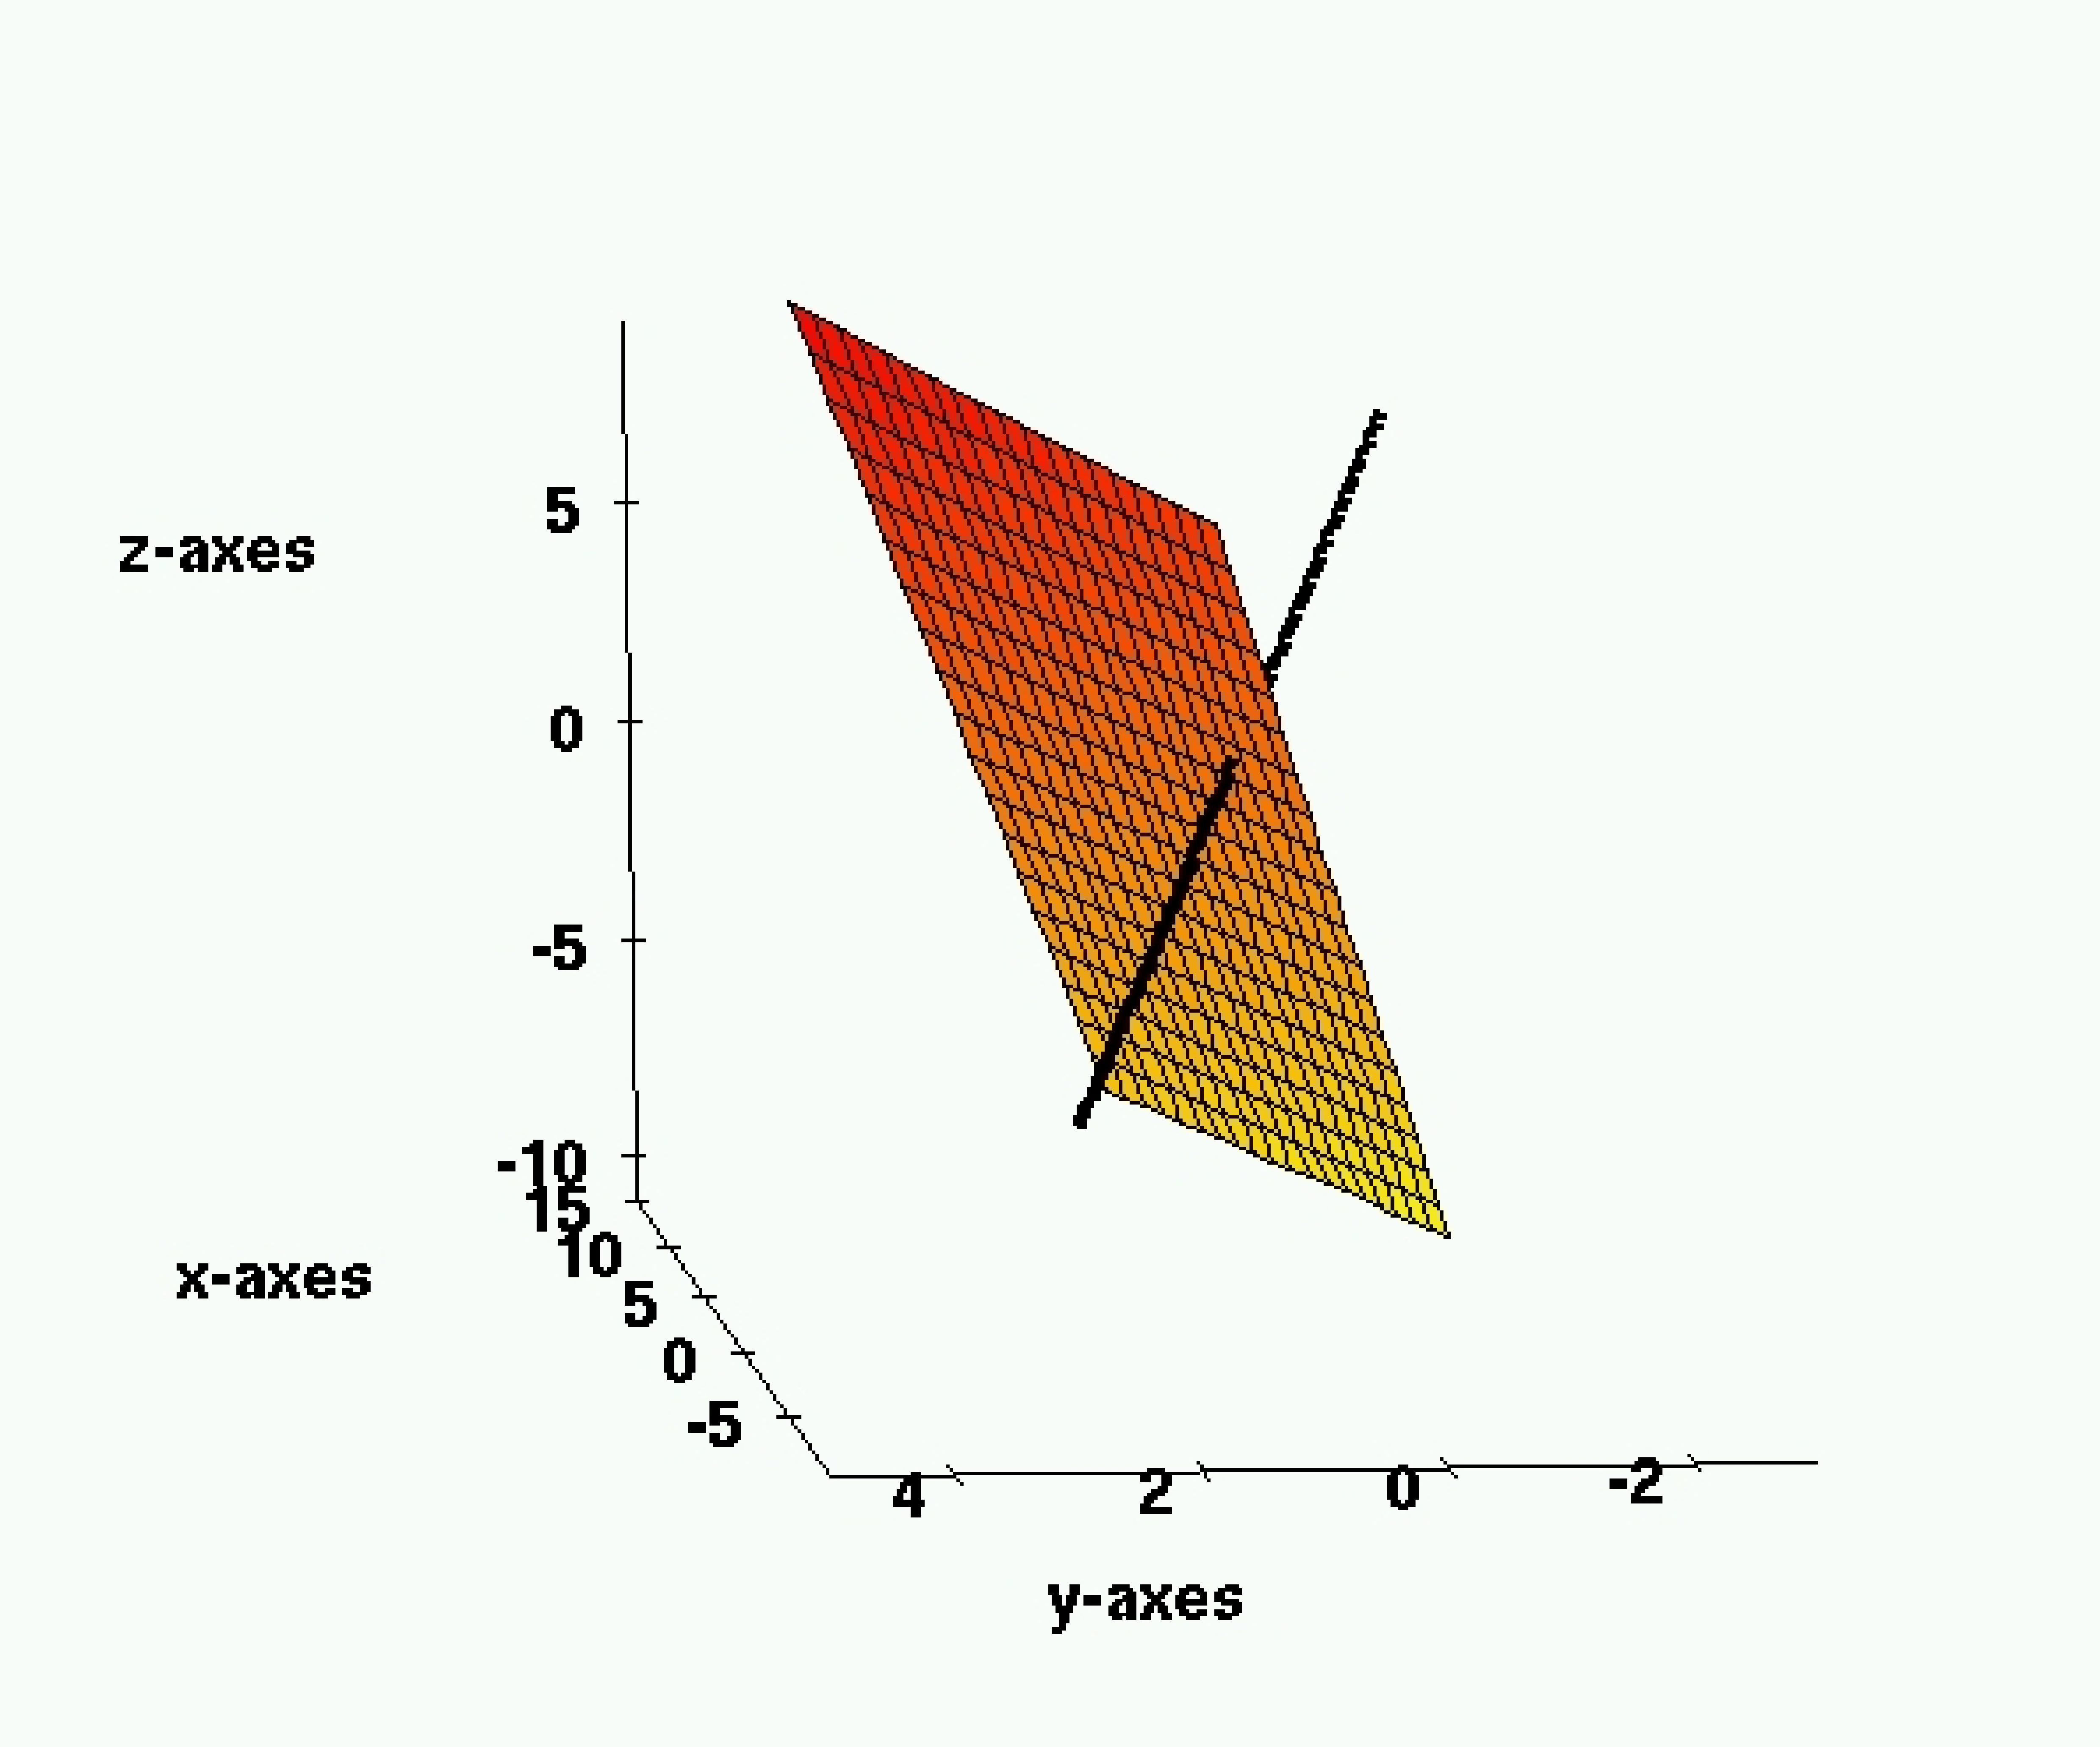
\includegraphics[width=0.7\textwidth]{figures/ebene2}
\end{center}
\end{frame}

\begin{frame}{Analytische Lösung}
Gleichsetzen ergibt: 
\[ 
\left ( \begin{array}{c}  2 \\ 1 \\ -1 \end{array} \right) +l 
\left ( \begin{array}{c}  1 \\ -1 \\ -1 \end{array} \right) +m
\left ( \begin{array}{c}  -3 \\ 1 \\ 4 \end{array} \right) = \left ( \begin{array}{c}  3 \\ 0 \\ 1 \end{array} \right) +k
\left ( \begin{array}{c}  4 \\ -1 \\ 2 \end{array} \right)
\] oder {
\[ 
\underbrace{\left(   
\begin{array} {ccc} 
1 & -3 & -4\\
-1 & 1 & 1 \\
-1 & 4 & -2  
\end{array} \right)}_{\displaystyle =:A} 
\underbrace{\left ( \begin{array}{c}  l \\ m \\ k \end{array}
  \right)}_{\displaystyle =:L} = \underbrace{\left ( \begin{array}{c}  1 \\ -1 \\ 2
  \end{array} \right)}_{\displaystyle =:b}
\] }
oder $A L=b$.
\end{frame}

\begin{frame}[fragile]{Definieren und Lösen des LGS}
\begin{itemize}
\item Definieren der Matrix $A$
\begin{sage}
>> A = matrix([[1,-3,-4],[-1,1,1],[-1,4,-2]]); A
\end{sage}
\begin{sage}
[ 1 -3 -4]
[-1  1  1]
[-1  4 -2]
\end{sage}
\item Definieren des Vektors $b$
\begin{sage}
>> b = vector([1,-1,2])
\end{sage}
\end{itemize}
\end{frame}

\begin{frame}[fragile]
\begin{itemize}
\item Lösen von  $A \ L=b$
\begin{sage}
A.solve_right(b)
\end{sage}
oder 
\begin{sage}
A\b
\end{sage}
ergibt
\begin{sage}
(6/5, 3/5, -2/5)
\end{sage}
\item Einsetzen in die Geradengleichung
\begin{sage}
>> x_s = matrix([g1,g2,g3]).subs(k=L[2]); x_s
\end{sage}
\begin{sage}
[7/5 2/5 1/5]
\end{sage}
\end{itemize}
\end{frame}

\begin{frame}[fragile]
\begin{itemize}
\item Matrizenoperationen
\begin{sage}
>> B = matrix([[1,0,0],[0,1,1],[1,1,1]])
>> A*B; A-B; A+B
\end{sage}
\begin{scriptsize}
\begin{sage}
[-3 -7 -7]  [ 0 -3 -4] [ 2 -3 -4]
[ 0  2  2]  [-1  0  0] [-1  2  2]
[-3  2  2]  [-2  3 -3] [ 0  5 -1]
\end{sage}
\end{scriptsize}
\item Berechnen der Inversen (mit Probe)
\begin{sage}
>> A^(-1), A*A^(-1)
\end{sage}
\begin{scriptsize}
\begin{sage}
[  -2/5 -22/15   1/15]
[  -1/5   -2/5    1/5]
[  -1/5  -1/15  -2/15]

[1 0 0]
[0 1 0]
[0 0 1]
\end{sage}
\end{scriptsize}
\end{itemize}
\end{frame}

%%%%%%%%%%%%%%%%%%%%%%%%%%%%%%
\subsection{Etwas Zahlentheorie}
%%%%%%%%%%%%%%%%%%%%%%%%%%%%%%%%%

\begin{frame}[fragile]{Etwas Zahlentheorie I}
Fermatsche Primzahlen: $F_n=2^{2^n} +1$. Finden Sie die kleinste
Zahl $F_n$, die keine Primzahl ist!
\begin{sage}
>> def F(n): return 2^(2^n)+1
>> [[F(m),is_prime(F(m))] for m in xrange(1,6) if is_prime (F(m))]
[[5, True], [17, True], [257, True], [65537, True]]
>> divisors(int(F(5)))
[1, 641, 6700417, 4294967297]
\end{sage}
\end{frame}

\begin{frame}[fragile]{Etwas Zahlentheorie II}
\begin{itemize}
\item Eine Liste der ersten  Primzahlen bis $100$
\begin{sage}
>> menge = set(range(1,101))
>> [m for m in menge if is_prime(m)]
oder >> filter(is_prime,menge)
\end{sage}
\begin{sage}
[2, 3, 5, 7, 11, 13, 17, 19, 23, 29, 31, 37, 41, 43, 47, 53, 59, 61, 67, 71, 73, 79, 83, 89, 97]
\end{sage}
\item Mersenne-Primzahlen $2^p-1$, $p$ Primzahl. Bestimmen der ersten
Mersenne Primzahlen im Bereich $\leq 200$.
\begin{sage}
>> menge = set(range(1,201))
>> primes = [m for m in menge if is_prime(m)]
>> [m for m in primes if is_prime(2^m-1)]
\end{sage}
\begin{sage}
[2, 3, 5, 7, 13, 17, 19, 31, 61, 89, 107, 127]
\end{sage}
\end{itemize}
\end{frame}

\begin{frame}[fragile]{Etwas Zahlentheorie III}
Wir geben für die natürlichen Zahlen $\leq 1000$ an, wieviele Zahlen
$1,2,3,\dots $ Teiler haben.
\begin{sage}
>> menge = set(range(1,1001))
>> liste = [number_of_divisors(int(m)) for m in menge]
>> for i in range(1,50):
>>     print (i,len([m for m in liste if m==i]))
\end{sage}

\begin{sage}
(1, 1)
(2, 168)
(3, 11)
(4, 292)
...
\end{sage}
Teiler der Zahl $840$:
\begin{sage}
>> divisors(840)
\end{sage}
\end{frame}

%%%%%%%%%%%%%%%%%%%%%%
\section{Nützliches und Hilfe}
%%%%%%%%%%%%%%%%%%%%%%%%%%%%%%%

\begin{frame}[fragile]{Überlebensregeln}
\begin{itemize}
\item Mehrere Befehle in einer Zeile durch {\color{blue} ';'} trennen. 
\item Bei Eingaben, die über mehrere Zeilen gehen, kann ein
  Zeilenumbruch durch {\color{blue} <ENTER>} erreicht werden.
\item Das Auswerten eines Blocks erfolgt mit {\color{blue} <SHIFT>+<ENTER>}.
\end{itemize}
\end{frame} 

\begin{frame}{Nützliches}
\begin{itemize}
\item {\color{blue} _ } refenziert die letzte Ausgabe.
\item Löschen aller eigenen Variablen und Zurücksetzen auf den Anfangsstatus: {\color{blue} reset()}
%\item Anzeigen aller definierten Variablen: {\color{blue} anames(All)}
%\item Anzeigen aller selbst definierten Variablen: {\color{blue} anames(All,User)}
\item profiler und debugger -> commandline
\item LaTex-doku ?
\item dokumentieren ? editor?
\end{itemize}
\end{frame}

\begin{frame}[fragile]{Hilfefunktionen in Sage}

\begin{itemize}
\item {\color{blue} Autocompletion :} mit der <TAB>-Taste erhält man alle möglichen Funktionen und/oder Variablen im gegebenen Kontext.
\item {\color{blue} \textit{command}? :} gibt ausführliche Hilfe zu \textit{command} an.
\item {\color{blue} help(\textit{command}) :} öffnet ein Hilfefenster zu \textit{command}.
\end{itemize}
\end{frame}
\end{document}





















